\documentclass{beamer}

\usepackage[utf8]{inputenc}
\usepackage[T1]{fontenc}
\usepackage[french]{babel}
\usepackage[ddmmyyyy]{datetime}

\usetheme{Warsaw}
\useinnertheme{rectangles}
\setbeamerfont{headline}{size=\large}
\setbeamerfont{frametitle}{size=\normalsize}

%Plan/Sommaire automatique avant chaque section
\AtBeginSection[]{
  \begin{frame}
  \frametitle{Plan}
  \tableofcontents[currentsection]
  \end{frame}
}

\author{Sonny Klotz - Jean-Didier Pailleux - Malek Zemni}
\institute{UVSQ}
\date{\today}
\usepackage{../tex/myInfolines}
\usepackage{longtable,array}
\title{Présentation Cahier des Charges}

\begin{document}

	\begin{frame}
		\titlepage
	\end{frame}
	
	\section*{Introduction}
		\begin{frame}
			Projet de L3 informatique UVSQ, remis par DCbrain.\\~\\
		\begin{itemize}
		\item Projet découlant d'un thème: le \textbf{Big Data}.\vspace{0.4cm}
		\item Analyse descriptives de données pour répondre au problème du \textbf{Big Data}.\vspace{0.4cm}
		\item Utilisation de graphe de flux par DCbrain pour visualiser le réseau (détections d'erreurs, optimisation).\vspace{0.4cm}
		\item \textbf{Objectif :} Fournir application web, outils permettent de charger des données, de les visualiser et les analyser.
		\end{itemize}
		\end{frame}
	
	\section{Architecture}
	\begin{frame}
		\begin{center}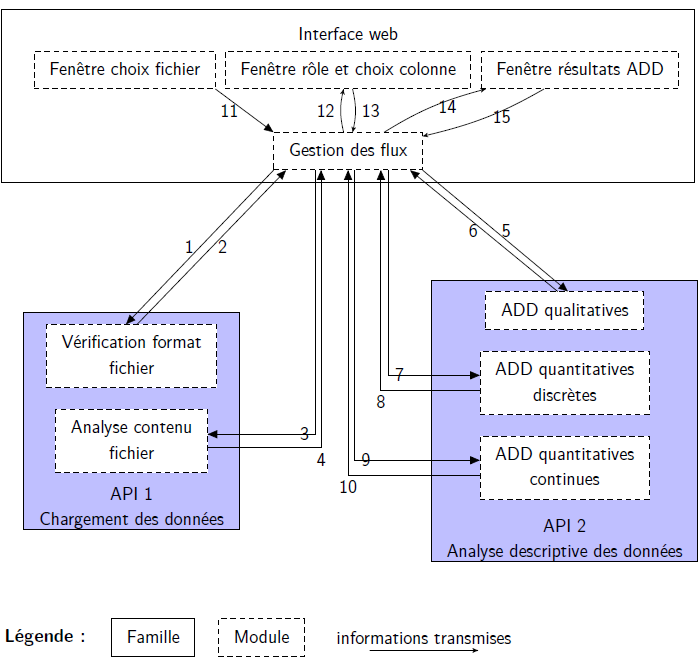
\includegraphics[scale=0.5]{org.png}\end{center}
	\end{frame}		
	
	\begin{frame}
		\begin{center}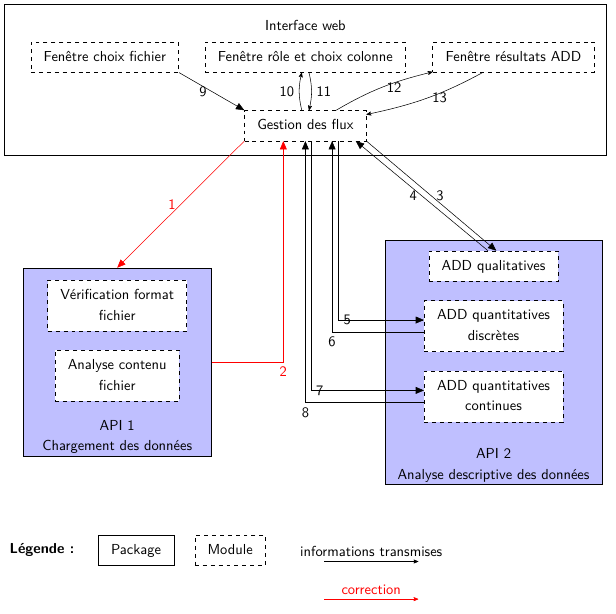
\includegraphics[scale=0.6]{org2.png}\end{center}
	\end{frame}
	
	\begin{frame}
		\textbf{API 1 :} Chargement des données\\
		\textit{Vérification format fichier :}
		\begin{itemize}
			\item Format csv
			\item Ouverture en lecture
			\item Texte brut ou formaté
		\end{itemize} \pause
		\vspace{1cm}
		\textit{Analyse contenu fichier :}
		\begin{itemize}
			\item Lecture des données du fichier ligne par ligne + stockage de ces données dans une \textbf{structure 1} 
			\item Description des données de chaque colonne : type, nom et données erronées + stockage dans une \textbf{structure 2}.
		\end{itemize}		 		
	\end{frame}
	
	\begin{frame}
		\begin{center}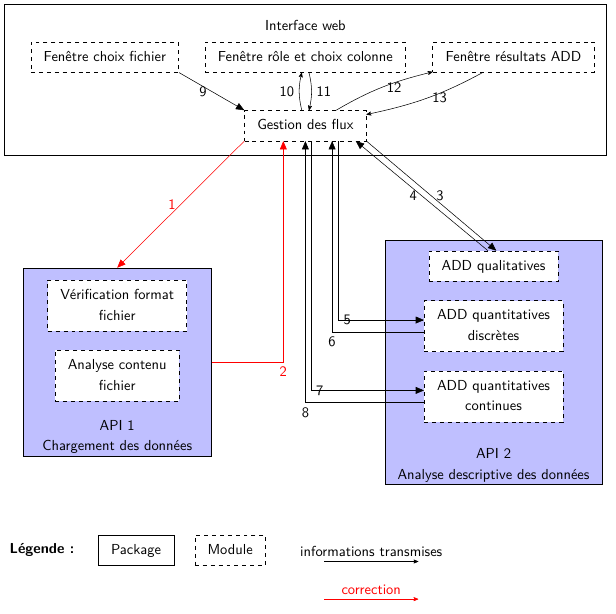
\includegraphics[scale=0.6]{org2.png}\end{center}
	\end{frame}
	
	\begin{frame}
		\textbf{API 2 :} Analyse descriptives des données\\
		\begin{itemize}
			\item \textbf{Données à analyser:} Données d'une colonne (Avec un possible filtrage).
			\item \textbf{Retours de l'analyse :} Informations statistiques et représentations graphiques.
			\item \textbf{ADD quantitatives continues :} Discrétisation des valeurs.
		\end{itemize}	
	\end{frame}
	
	\begin{frame}
		\begin{center}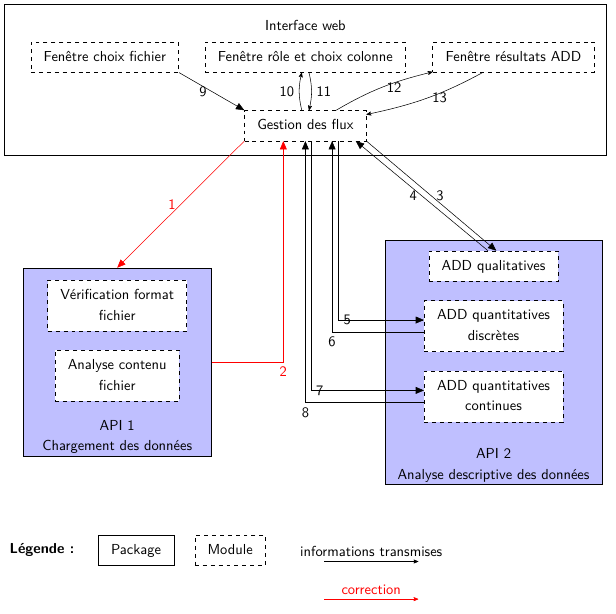
\includegraphics[scale=0.6]{org2.png}\end{center}
	\end{frame}
	
	\begin{frame}
		\textbf{Interface web}\\
		\textit{Gestion des flux :}
		\begin{itemize}
			\item \textbf{Flux d'exécution :} Gestion des branchements et arrêts de l'application en cas d'erreur(s).
			\item \textbf{Flux de données :} Rôle d'interface pour communiquer les données entre les différents modules
		\end{itemize} \pause
		 \vspace{1cm}
		 
		\textit{Fenêtre choix fichier :}
		\begin{itemize}
			\item \textbf{Choix du fichier :} Parcours de l'arborescence de fichiers - Drag\&Drop.
		\end{itemize}
	\end{frame}
	
	\begin{frame}
		\textit{Fenêtre rôle et choix colonne :}
		\begin{itemize}
		\item Affiche sous forme d'un tableau : nom des colonnes - nombre de lignes et de colonnes - un échantillon grâce à une navigation.
		\item Affichage des données erronés + description.
		\item Sélection et envoi d'une colonne de mesures pour analyse. 
		\end{itemize} \pause
		 \vspace{1cm}
		 
		\textit{Fenêtre résultats ADD :}
		\begin{itemize}
		\item Affichage des résultats d'analyse descriptive : informations statistiques + représentations graphiques.
		\item Fonctionnalité de retour en arrière pour analyser une nouvelle colonne.
		\item Fonctionnalité de téléchargement des résultats au format \lstinline!.csv!
		\end{itemize}
	\end{frame}
	
	\section{Outils, langages de programmation} 
		\begin{frame} 
			\textbf{Contraintes :} sur le produit :
			\begin{enumerate}
				\item Fournir une application web.
				\item Développé avec un langage de programmation compatible avec l’analyse de données.
				\item Fournir des API pour le chargement et l’analyse de données.
			\end{enumerate}
			~\\~\\
			\pause
			\textbf{Outils et langages de programmation}
			\begin{itemize}
				\item \textbf{Python :} adapté pour l’ADD et le développement d’applications web
				\item \textbf{Flask :} framework web Python
				\item \textbf{HTML et CSS :} présentation et mise en forme des pages web
				\item \textbf{JavaScript :} dynamiser les pages web
				\item \textbf{jQuery :} gestion des événements et \textbf{Ajax}
				\item \textbf{c3js :} module de représentations graphiques
				\item \textbf{Sphinx :} framework Python, génération de documentation
			\end{itemize}
		\end{frame}
	
	\section{Fonctionnement de l'application}
		\begin{frame}
			\textbf{Fichier CSV :} contenu structuré établi par le client : décrit par des colonnes aux types prédéfini
			\begin{center}\vspace{-1.2em}\footnotesize\begin{longtable}{|>{\centering}m{4cm}|>{\centering}m{1cm}|>{\centering}m{1cm}|>{\centering}m{2cm}|>{\centering\arraybackslash}m{2cm}|}			
				\hline \multicolumn{1}{|c|}{\textbf{timestamp}} & \multicolumn{1}{c|}{\textbf{parent}} & \multicolumn{1}{ c|}{\textbf{enfant}} & \multicolumn{1}{c|}{\textbf{mesure 1}} & {\textbf{mesure 2}} \\
				\hline 	January 1st 2017, 15:00:00.000 & 102 & 95 & 26644.235 & 176.253\\
				\hline
			\end{longtable}\end{center}
			\pause
			~\\
			API chargement de données gère des fichiers CSV quelconques :
			\begin{itemize}
				\item Lignes avec données en moins ou en trop
				\item Colonnes désordonnées
				\item Délimiteur quelconque
			\end{itemize}
		\end{frame}
		
		\begin{frame}
			\textbf{Interface web :} gère l'interaction avec l'utilisateur
			\begin{enumerate}
				\item Importation du fichier CSV
				\item Visualisation du contenu + erreurs
				\item Application de filtres + attribution rôles colonnes
				\item Envoi d'une colonne pour l'analyse
				\item Affichage des résultats de l'analyse : graphes et valeurs statistiques
				\item Téléchargement des résultats de l'analyse
			\end{enumerate}
			~\\~\\
			\pause
			\textbf{APIs :} réutilisables par le client, gèrent le traitement des données
			\begin{itemize}
				\item \textbf{Chargement de données :} préparation du contenu du fichier pour l'affichage
				\item \textbf{Analyse descriptive des données :} analyse des colonnes du fichier
			\end{itemize}
		\end{frame}
	
	\section{Bilan technique}
		\subsection*{Points délicats}
		\begin{frame}
			\textbf{Paradigme client / serveur}\\
				\begin{center}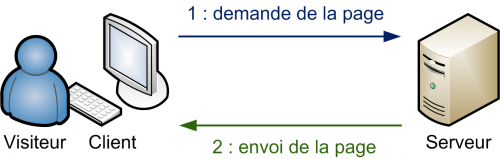
\includegraphics[scale=0.5]{clientServeur.png}\end{center}
				\begin{itemize}
				\item \textbf{Client} : Navigateur Web -> Requête URL au Serveur.
				\item \textbf{Serveur} : Réception de la requête -> retour de la page demandée.
				\item \textbf{Flask} : framework web choisi.
				\end{itemize}
		\end{frame}
		
		\begin{frame}
			\textbf{Templates HTML}\\
				\begin{center}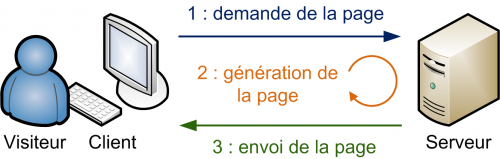
\includegraphics[scale=0.4]{langageServeur.png}\end{center}
				\begin{itemize}
				\item \textbf{Template} : Page html formatée générique, avec des balises.
				\item \textbf{Flask} :\\
					Création de la page html finale.\\
					Balises peuvent contenir du code Python.
				\end{itemize}
				\begin{block}{Enjeux}
				Pages dynamiques - Circulation des données.
				\end{block}
		\end{frame}
		
		\begin{frame}
		%image a modifier sur paint
			\textbf{Les applets}\\
				\begin{center}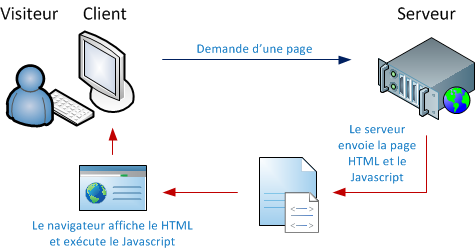
\includegraphics[scale=0.5]{applet.png}\end{center}
				\begin{enumerate}
				\item Balises <script> pour HTML.
				\item Code exécuté côté client : \textbf{\textit{JavaScript}}
				\end{enumerate}
				
				\textbf{Dynamisme} : Animations, programmation évènementielle, Html modifié en direct.
				
				\begin{block}{Enjeu}
				Circulation des données nécessaire : Côté client <=> Côté serveur.
				\end{block}
		\end{frame}
		
		\begin{frame}
		%image a modifier sur paint
			\textbf{Ajax} (Asynchronous JavaScript and Xml)\\
				\begin{center}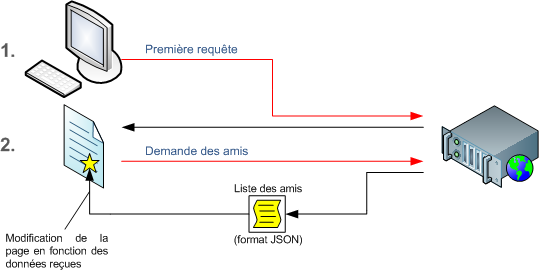
\includegraphics[scale=0.5]{ajax.png}\end{center}
				
				\begin{itemize}
				\item Rafraichissement \textbf{partiel} de la page.\\ %Requete, ne renvoie pas toute une page
				\item JSON : syntaxe des objets JavaScript, légère. \\ 
				\item Mécanisme asynchrone : fonctions \textbf{callback}
				\end{itemize}
		\end{frame}
		
		\subsection*{Problèmes rencontrés}
		\begin{frame}
			\begin{itemize}
			\item \textbf{Divergence avec les spécifications}\\
				\hspace{1em} Problème : Utilisation des fichiers.\\
				\hspace{1em} Caractéristique : Indépendance ressources Client / Serveur.\\
				\hspace{1em} Solution : envoi Ajax.\vspace{1em} \pause
				
			\item \textbf{Séries temporelles}\\
				\hspace{1em} Problème : Affichage incohérent.\\
				\hspace{1em} Caractéristique : Plusieurs mesures à un temps donné.\\
				\hspace{1em} Solution : Une série temporelle par arc distinct.\vspace{1em} \pause
				
			\item \textbf{Performances (non résolu)}\\
				\hspace{1em} Problème : Affichage du jeu de données.\\
				\hspace{1em} Caractéristique : Complexité non-linéaire.\\
				\hspace{1em} Solution (éventuelle) : Module JavaScript personnel.\pause
			\end{itemize}
		\end{frame}
	
	\section{Organisation interne du groupe}
		\begin{frame}
			\begin{center}\vspace{-1em}\footnotesize\begin{longtable}{|>{\centering}m{4.5cm}|>{\centering}m{1.5cm}|>{\centering}m{1.5cm}|>{\centering\arraybackslash}m{2cm}|}
			\hline \multicolumn{1}{|c|}{\textbf{Module}} & \multicolumn{1}{c|}{\textbf{Malek}} & \multicolumn{1}{ c|}{\textbf{Sonny}} & \multicolumn{1}{c|}{\textbf{Jean-Didier}}\\
			\hline 	Gestion des flux & ~ & ~ & x\\
			\hline 	Fenêtre choix fichier & ~ & ~ & x\\
			\hline 	Fenêtre rôle et choix colonne & x & ~ & ~\\
			\hline 	Fenêtre résultats ADD & ~ & x & ~\\
			\hline  ADD qualitatives & ~ & ~ & x\\
			\hline 	ADD quantitatives discrètes & ~ & x & ~\\
			\hline 	ADD quantitative continues &  ~ & x & ~\\
			\hline 	Vérification format fichier & x & ~ & ~\\
			\hline 	Analyse contenu fichier & x & ~ & ~\\
			\hline
			\end{longtable}\vspace{-2.2em}\end{center}
			
			\begin{itemize}
			\item Groupe de trois personnes.
			\item Planning respecté.
			\item Travail en groupe.
			\end{itemize}
		\end{frame}
	
	\section{Coûts}
		\begin{frame}
			\begin{center}\vspace{-1em}\footnotesize\begin{longtable}{|>{\centering}m{3cm}|>{\centering}m{3cm}|>{\centering\arraybackslash}m{1.5cm}|}			
			\hline \multicolumn{1}{|c|}{\textbf{Module}} & \multicolumn{1}{c|}{\textbf{Estimation}} & \multicolumn{1}{c|}{\textbf{Coût final}}\\
			\hline 	Gestion des flux & 15 & \textbf{98}\\
			\hline 	Fenêtre choix fichier & 30 & \textbf{72}\\
			\hline 	Fenêtre rôle et choix colonne & 65 & \textbf{180}\\
			\hline 	Fenêtre résultats ADD & 100 & \textbf{200}\\
			\hline  ADD qualitatives  & 60 & 53\\
			\hline 	ADD quantitatives discrètes & 100 & 89\\
			\hline 	ADD quantitatives continues & 85 & 93\\
			\hline 	Vérification format fichier & 30 & 35\\
			\hline 	Analyse contenu fichier & 60 & 70\\
			\hline \textbf{Coût Total} & \textbf{545} & \textbf{850}\\
			\hline 	
			\end{longtable}\vspace{-2.2em}\end{center}
		\end{frame}
		
		\begin{frame}
			\begin{block}{Justifications}
			\vspace{1em}
			\textbf{Ajax} : Charge supplémentaire code.\\
			\vspace{1em}
			\textbf{Séries temporelles} : Deux fonctionnalités supplémentaires.\\
			\vspace{1em}
			\textbf{Filtrage des valeurs} : Demandées après l'écriture du cahier des charges.
			\vspace{1em}
			\end{block}
		\end{frame}
	
	\section{Conclusion}
		\begin{frame}
			\underline{\textbf{Support}} :\\
				\hspace{1em}Masse de données collectées sur un \textbf{\textit{réseau physique}} assimilé à un \textbf{\textit{graphe de flux}}.\\
			\vspace{1em}
			\underline{\textbf{Applet}} :\\
				\hspace{1em}Traitement des données à l'aide d'analyses descriptives.\\
				\hspace{1em}Résultats : statistiques et visuels.\\
			\vspace{1em}
			\underline{\textbf{Améliorations possibles}} :\\
				\hspace{1em}Interface-web : performances de l'affichage.\\
				\hspace{1em}API extensibles :
					\hspace{1em}\begin{itemize}\item ADD : analyses multidimensionnelles et nouvelles représentations graphiques.\end{itemize}
		\end{frame}
	
\end{document}
